\apendice{Documentación de usuario}

\section{Introducción}
En esta sección se detallan los requerimientos de la aplicación, los pasos de instalación, despliegue, así como las indicaciones para su uso adecuado.
\section{Requisitos de usuarios}
Los requesitos para poder hacer uso de la aplicación son:
\begin{itemize}
    \item Tener instalado Python (minimo la version 3.7) y el resto de las librerías contenidas en el \textit{requeriments.txt}.
    \item Tener un navegador web compatible con HTML5 
\end{itemize}

\section{Instalación}
Instalar el contenedor docker de la aplicación.

\section{Manual del usuario}
En esta sección se explicarán las diferentes tareas que puede hacer un usario en la aplicación.
\imagen{homeAPP}{\textit{Home} de la aplicación}
\subsection{Carga de modelo de detección}
Esta opción se encuentra en el \textit{home} de la aplicación, correspondiendose esta opción con el primer botón, al hacer \textit{click} sobre él se nos abrirá una modal, la cuál cuenta con dos inputs, uno de tipo text y otro de tipo file(este posee funcionalidad de \textit{click} y de \textit{drag and drop}).
\begin{figure}[!h]
    \centering
    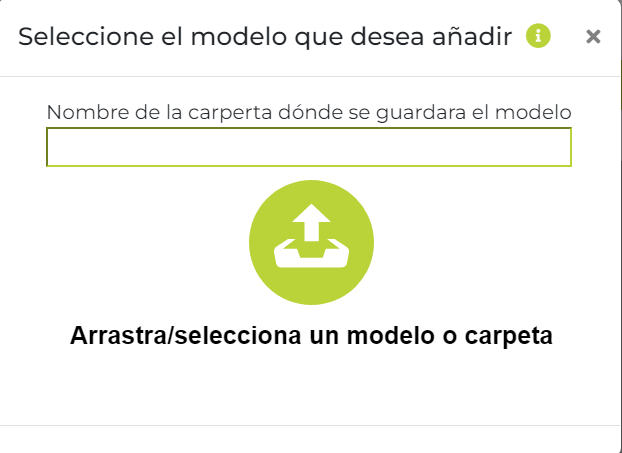
\includegraphics[width=0.6\textwidth]{modalModel}
    \caption{Modal de añadir modelos}\label{fig:modalModel}
\end{figure}
El input de tipo \textit{text}, sirve para introducir el nombre de la carpeta en la cuál se guardará el modelo de detección, de tal forma que sea más fácil encontrarlo posteriormente.
En segundo input de tipo \textit{file}, nos permite escoger el modelo que queremos añadir a la aplicación, ya sea un modelo de \textit{Tensorflow Lite} o una carpeta con el modelo de \textit{Tensorflow}.
\subsection{Carga de fichero de etiquetas}
\subsection{Cambiar modelo de detección}
\subsection{Cambiar fichero de etiquetas}
\subsection{Detección de objetos en una imagen}
\subsection{Detección de objetos en un vídeo}
\subsection{Contabilizar objetos en un vídeo}
\subsection{Detección de objetos a tráves de la URL de una imágen}
\subsection{Detección de objetos a tráves de la URL de un vídeo de YouTube}
\subsection{Detección de objetos a tráves de webcam}
